\subsection{Introduction}

Ice sheets are key components of Earth's climate system. They contain
nearly all of the planet's fresh water, changes in their volume have an
immediate effect on sea level, changes in their area and surface
characteristics affect global albedo, and they play a role in the
circulation of both the atmosphere and the ocean. Through the latter
half of the Quaternary, ice sheets have modulated the planetary response
to orbitally-driven insolation cycles. Looking forward, the Greenland
and Antarctic ice sheets have the potential to play important roles in
climate change.

A numerical model is a discrete approximation of a continuous process.
The approximation is discrete due to the finite nature of a computer's
precision. The underlying process is continuous because it is commonly
formulated in terms of partial or ordinary differential equations.
Numerical models can not be solved until the boundary conditions and
initial conditions are specified. Such models may be very simple such as
a \href{Wikipedia:Harmonic oscillator}{Wikipedia:Harmonic oscillator},
or very complex, as in a
\href{Wikipedia:Global climate model}{Wikipedia:Global climate model}.

The model we will use is called CISM. It has its basis in a set of
programs and climate ``drivers'' built over many years by a research
group at the \href{http://www.bris.ac.uk/}{University of Bristol}, led
by Tony Payne. Historically, the effort was called
\href{http://forge.nesc.ac.uk/projects/glimmer/}{Glimmer}. More
recently, a collaborative project has extended the effort in many novel
and exciting ways. This is called the Community Ice Sheet Model, or
\href{http://websrv.cs.umt.edu/isis/}{CISM}.

\subsection{Conservation equations}

The mathematical descriptions of physical systems we encounter in Earth
science problems begin from statements requiring the conservation of
energy, momentum, or mass.

\subsubsection{Integral form}

The mathematical formulation of conservation can be arrived at by
considering the change in a quantity $\phi$ that is known in a
\textbf{control} volume $V$. The
\href{Wikipedia:control volume}{Wikipedia:control volume} is enclosed by
a surface $S$, with outward positive unit vector $\hat n$ normal to $S$.


\begin{figure}
  \begin{center}
    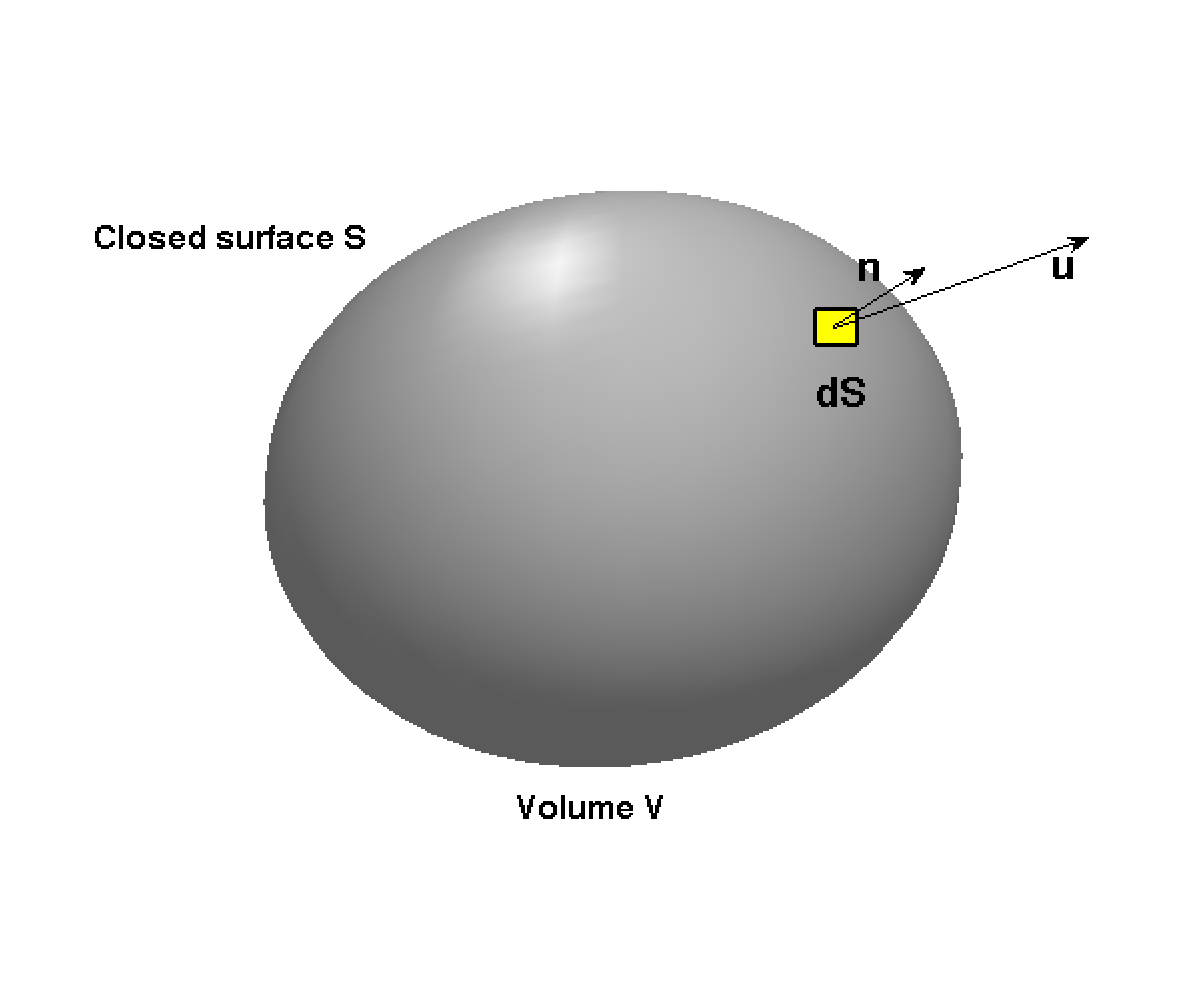
\includegraphics[width=0.9\columnwidth]{\dir/figs/ControlVolume.eps}
  \end{center}
  \caption{Diagram of control volume and associated quantities.}
  \label{fig:controlvol}
\end{figure} 


The value of $\phi$ within $V$ may change over time if

\begin{enumerate}
\itemsep1pt\parskip0pt\parsep0pt
\item
  there is a flux through $S$. The flux is partitioned into two parts,
  one due to \url{Wikipedia:diffusion} and another due to
  \url{Wikipedia:advection}.
\item
  Creation or destruction of $\phi$ within $V$.
\end{enumerate}

Formally, time rate of change in $\phi$ within $V$ is written:

$
{\frac{ \partial }{ \partial t}} { \int }_{ V} \phi dV~ = ~ -{ \int }_{ S} {\mathbf F}
    {\cdot} \hat n~ dS~ - ~{ \int }_{ S} \phi {\mathbf u} {\cdot} \hat n ~ dS~
    + ~{ \int }_{ V} HdV
$

where ${\mathbf F}$ represents the flux due to diffusion
($\mathbf{F} \propto \nabla \phi$), $\phi {\mathbf u}$ represents
velocity field \emph{\href{Wikipedia:advection}{advecting}} $\phi$, $H$
represents a source (or sink) of $\phi$. Vector quantities are
represented in \textbf{boldface}. The negative signs in front of the
first two terms on the right-hand side indicate that an outward flux
results in decrease of $\phi$ in the volume enclosed by $S$.

This statement of conservation of $\phi$ in the unit volume $V$ is
always true, independent of the size of $V$ and even if the fields
enclosed by $S$ are not continuous. This is the case because we
integrate over $V$. It is important to note that that information on
spatial scales smaller than $V$ is lost in the integration.

\subsubsection{Derivative form}

Numerical models are often easier to formulate from the derivative form
of the conservation equation. This requires the derivatives of $\phi$ to
exist within $V$. This requirement allows the integral form of the
conservation equation to be written as partial differential equations
which are upheld with in the control volume.

Begin with the terms describing diffusive and advective fluxes into or
out of the control volume. The
\href{Wikipedia:divergence theorem}{Wikipedia:divergence theorem} states
that

$
{ \int }_{S} {\mathbf F} {\cdot} \hat{n} ~dS~ = ~{ \int }_{V} \nabla 
    {\cdot} {\mathbf F} ~dV. 
$

Or, adapting the notation that the subscript indicates a single
component of a vector, and that repeated subscript indices in a single
term are to be summed,

$
{ \int }_{ S} {\mathbf F}_{ j} ~n_{ j} ~dS~ = ~{ \int }_{ V} {\frac{
    \partial {\mathbf F}_{ j} }{ \partial x_{ j} }} ~dV.
$

Using the divergence theorem, the surface integrals over fluxes may be
replaced,

$
-{ \int }_{ S} {\mathbf F} {\cdot} \hat{n}dS~ - ~{ \int }_{ S} \phi {\mathbf u}
    {\cdot}\hat{n} dS~ = ~ -{ \int }_{ V} \nabla {\cdot} \left ( {
    {\mathbf F}~ + ~ \phi ~ {\mathbf u}} \right )dV.
$

Assuming that the coordinate system is stationary with respect to the
velocity field $\mathbf{u}$ (Eularian reference frame), it is possible
to write

$
{\frac{ \partial}{ \partial t}} { \int }_{ V} \phi ~dV~ = ~{ \int }_{ V}
    {\frac{ \partial \phi }{ \partial t}} ~dV~
$

The end result is that the integral form of the conservation equation
can now be written

$
{ \int }_{ V} \left\{ {{\frac{ \partial \phi }{ \partial t}}
    ~ + ~ \nabla {\cdot} \left ( { {\mathbf F}~ + ~ \phi {\mathbf u}} \right ) ~
    - ~ H} \right\} dV~ = ~ 0
$

Because $V$ is an arbitrary volume, this equation can only be true if
the term in brackets is zero for the volume. Hence, for any volume
having continuously differentiable $\phi$,

$
{\frac{ \partial \phi }{ \partial t}} ~ + ~ \nabla {\cdot} 
    \left ( { {\mathbf F}~ + ~ \phi {\mathbf u}} \right ) ~ - ~H~ = ~ 0.
$

This is the general form for all conservation laws in continuum
mechanics.

\subsubsection{Applications of the conservation equation}

Having established a generalized conservation law, it is now applied to
the three quantities which are conserved in an ice sheet model; mass,
energy, and momentum.

\paragraph{Conservation of mass}

In this case $\phi$ is the mass $M$, or more conveniently
$M = \int_V \rho dV$, the integral of the density over the volume.
Assuming that there are no sources or sinks of mass in the volume ($H$ =
0), the conservation equation is written

$
\int_{V}\frac{\partial \rho} {\partial t} ~dV ~+~ \int_{V} \nabla \cdot \rho \mathbf{u} dV~=~0
$

Ice is incompressibile, meaning that the density does not change in
time, and the equation for local mass continuity is

$
\nabla \cdot \mathbf{u} ~=~0.
$

Applying the $\nabla$ operator in a cartesian coordinates produces

$
\frac{\partial u_{x}}{\partial x}~+~\frac{\partial u_{y}}{\partial y} ~+\frac{\partial u_{z}}{\partial z}~=~0.  
$

To make use of this statement, we need to integrate

$
\int_{b}^{s} \left( \frac{\partial u_{x}}{\partial x}~+~\frac{\partial u_{y}}{\partial y} ~+\frac{\partial u_{z}}{\partial z}\right) dz~=~0  
$

from the base $b$ to the upper surface $s$ of the ice mass. The integral
of $\frac{\partial u_z}{\partial z}$ is simply the difference between
the vertical component of the velocity at the upper and lower surfaces,
so

$
u_{z} \left(s\right)-u_{z} \left(b\right)~=~-\int_{b}^{s} \frac{\partial u_{x}}{\partial x} dz ~-~\int_{b}^{s} \frac{\partial u_{y}}{\partial y} dz  
$

Changing the order of integration using Leibnitz rule

$\begin{matrix}
u_{z} \left(s\right)-u_{z} \left(b\right) & = & -~\frac{\partial}{\partial x} \int_{b}^{s} u_{x} dz ~ +~u_{x}(s)\frac{\partial s}{\partial x} ~-~ u_{x}(b)\frac{\partial b}{\partial x}  \\ 
& & -~\frac{\partial}{\partial y}\int_{b}^{s} u_{y} dz   ~ +~u_{y}(s)\frac{\partial s}{\partial y} ~-~ u_{y}(b)\frac{\partial b}{\partial x}
\end{matrix}$

The vertical velocity at the upper surface is the result of motion down
the surface slope, the rate of new accumulation $\dot{a}$ and any
time-change in surface height

$
u_{z} \left(s\right)~=~\frac{\partial s}{\partial t}~+~u_{x}(s)\frac{\partial s}{\partial x}~+~u_{y}(s)\frac{\partial s}{\partial y}~-~\dot{a} 
$

recognizing that a negative accumulation rate indicates ablation.
Similarly, the vertical velocity at the lower surface is

$
u_{z} \left(b\right)~=~\frac{\partial b}{\partial t}~+~u_{x}(b)\frac{\partial b}{\partial x}~+~u_{y}(b)\frac{\partial b}{\partial y}~-~\dot{b} 
$

in which $\dot{b}$ represents the basal accumulation rate.

Substituting equations we find that many terms cancel

$
\frac{\partial s}{\partial t}~-~\dot{a}~-~\frac{\partial b}{\partial t}~+~\dot{b}~=~-~\frac{\partial}{\partial x} \int_{b}^{s} u_{x} dz~-~\frac{\partial}{\partial y} \int_{b}^{s} u_{y} dz
$

Finally, making the simplification $h=s-b$ we have

$
\frac{\partial h}{\partial t}~=~-~\frac{\partial}{\partial x} \int_{b}^{s} u_{x} dz~-~\frac{\partial}{\partial y} \int_{b}^{s} u_{y} dz ~+~\dot{a}~-~\dot{b}
$

The vertically-integrated form

$
\frac{\partial h}{\partial t}~=~-~\nabla \cdot \left( U_{i} h \right) +~\dot{a}~-~\dot{b}
$

in which $U_{i}$ represents the vertically averaged velocity, i.e.
$U_i = \frac{1}{h}\int_{b}^{s}u_{i}dz$ . This equation is prognostic. We
use the current geometry of the ice to compute a future time-change in
that geometry.

\paragraph{Conservation of energy}

The first law of thermodynamics is used to make a basic statement of
conservation of energy in a volume of ice V within a surface S is

$
\frac{d}{d t} \int_{V}E ~dV~=~- \int_{S}\mathbf{F}\cdot \hat{n}~dS~-~\int_{S}E \mathbf{u}\cdot \hat{n}~dS~+~\int_{V}W dV
$

in which $E$ represents the energy of the volume, $F_{i}$ is a flux due
to diffusion, and $W$ represents any sources or sinks of energy within
the volume. The term $Eu_{i}$ is a flux through $S$ due to advection.
Following the steps laid out earlier, we use the divergence theorem and
the assumptions of continuous fields and incompressibility, such that

$
\frac{dE}{dt}~+~\nabla \cdot \left(F_{i} +E u_{i}  \right)~-~W~=~0
$

Our goal is to use the first law of thermodynamics in order to compute
the temperature of the ice and any change it may undergo over time.

The energy $E$ is the product of density and the specific internal
energy of the ice $e$, which is itself the product of the specific heat
capacity $c_{p}$ and temperature $T$ because there is no transfer
between internal energy and pressure for an incompressible fluid. Thus,

$\begin{matrix}
\frac{dE}{dt}&=&\frac{d\left(\rho e \right)}{dt} \\
&=&\rho\frac{de}{dt}~+~e \frac{d\rho}{dt}\\
&=&\rho c_{p} \frac{dT}{dt}
\end{matrix}$

The flux due to diffusion follows Fourier's ``law'' for heat conduction
so

$\begin{matrix}
\nabla \cdot F_{i}&=&\nabla \cdot \left( -k ~\nabla T  \right) \\
&=&-k~\nabla^{2}T
\end{matrix}$

in which $k$ represents the thermal diffusivity of ice and we assume
gradients in its magnitude to be negligible.

Using progress made above and assuming that $\nabla \cdot u_{i}$ is
small with respect to other terms, we can write the advection term

$\begin{matrix}
\nabla \cdot \left(E u_{i} \right)~=~\rho c_{p}~ u_{i} \cdot \nabla T  
\end{matrix}$

Two quantities must be considered as energy sources, the work done on
the system by internal deformation and the latent heat associated with
phase changes. The former is the product of strain rate and the
deviatoric stress $\dot{\epsilon}_{ij} \tau_{ij}$. The latter is the
product of the latent heat of fusion and the amount of material subject
to melting (freezing) per unit volume per unit time, $L_{f}M_{f}$.

At last, we are able to write equation
\textbackslash{}ref\{equation:enbal2\} in terms of temperature

$
\frac{\partial T}{\partial t}~=~\frac{k}{\rho c_{p}} \nabla^{2}T~-~u_{i}\cdot \nabla T~+~\frac{1}{\rho c_{p}} \dot{\epsilon}_{ij} \tau_{ij} ~+~\frac{1}{\rho c_{p}} L_{f} M_{f}
$

It is often the case that horizontal terms
$\frac{\partial^{2} T}{\partial x^{2}}$ and
$\frac{\partial^{2} T}{\partial y^{2}}$ are small enough to be ignored.

\paragraph{Conservation of momentum}

Starting from Newton's second law of motion, conservation of momentum is

$
\frac{d} {dt} \int_{V}\rho u_{i}~dV ~ = ~ \int_{V} \frac{\partial \sigma_{ij}} {\partial x_{j}} ~dV +  \int_{V} \rho g_{i}~dV
$

where $t$ represents time, $\rho$ represents density, $u$ represents
velocity, $\sigma_{ij}$ represents the stress tensor, $g$ represents the
acceleration due to gravity, $V$ represents the volume of an arbitrary
fluid element, and $(i,j)= \{x, y, z\}$ in a cartesian coordinate
system. Equation \textbackslash{}ref\{equation:mobal1\} tells us that a
fluid element of arbitrary size experiences a ``body force''
$\rho g_{i}\delta V$ due to gravity and a force
$\frac{\partial \sigma_{ij}} {\partial x_{j}} \delta V$ due to the
surrounding fluid.

Making the assumptions that we have continuous fields and that ice is
incompressible (that is, its density $\rho$ does not change under
conditions of interest to us), we can write

$
\rho \frac{D u_{i}}{D t}~=~\frac{\partial \sigma_{ij}}{\partial x_{j}} + \rho g_{i}
$

in which $D$ is a material derivative. Due to the fact that Froude
number \href{Wikipedia:Froude number}{Wikipedia:Froude number} for ice
flow is extremely small, the acceleration term (the first term on the
left hand side) could be neglected and we arrive to a steady-state form.

$
\frac{\partial \sigma_{ij}}{\partial x_{j}} + \rho g_{i} ~=~0
$

We are left with the very simple statement that the gravitational
driving force is balanced by forces resulting from the stresses
$\sigma_{ij}$.

The stress tensor $\sigma_{ij}$ has nine components in our three
dimensional cartesian coordinate system

$
\mathbf{\sigma} =
\left\vert  \begin{array}{ccc} 
    \sigma _{ xx} & \sigma _{ xy} & \sigma _{ xz} \\
    \sigma _{ yx} & \sigma _{ yy} & \sigma _{ yz} \\
    \sigma _{ zx} & \sigma _{ zy} & \sigma _{ zz} \\
\end{array} \right\vert 
$

The components along the diagonal are called normal stresses and the
off-diagonal components are called shear stresses. Deformation results
not from the full stress but from the deviatoric stress

$
\tau_{ ij} ~ = ~ \sigma _{ ij} ~ - ~{\frac{ 1}{ 3}} \sigma _{ kk} \delta _{ ij}
$

in which $\delta_{ ij}$ is the Kroneker delta.

\subsubsection{Constitutive relationship}

Strain rates $\dot{\epsilon}_{ij}$ are related to the stress tensor
$\tau_{ij}$ by the generalized Glen flow law

$
\dot{\epsilon}_{ij}~=~A(T^{*})\tau_{e}^{n-1}\tau_{ij}
$

in which $T^{*}$ is the absolute temperature corrected for the pressure
dependence of the melt temperature, $\tau_{e}$ is the second invariant
of the stress tensor and the exponent $n$ is 3. The rate factor $A$
follows the Arrhenius relationship

$
A\left( T^{*}\right)~=~E A_{o}e^{-Q/RT^{*}}
$

in which $A_{o}$ is a constant, $Q$ represents the activation energy for
crystal creep, $R$ is the gas constant, and $E$ is a tuning parameter
used to account for the effects of impurities and anisotropic ice
fabrics. The homologous temperature is

$
T^{*}=T+\rho g H \Phi
$

in which $\Phi$ is 9.8 $\times$10$^{-8}$ K Pa$^{-1}$, about 8.7
$\times$10$^{-4}$ K m$^{-1}$. The pressure-dependent melt temperature is
simply the triple point temperature less the product $\rho g H \Phi$.

\subsection{Numerical solutions of field equations}

3D, thermo-mechanically coupled ice sheet models. 3D refers to the
explicit vertical layering of the model for computing temperature.
Thermo-mechanical means that the ice viscosity is sensitive to
temperature, and an iterative procedure must be used to find the flow
rates from temperature. Both models exploit the often used shallow ice
approximation \textbackslash{}citep\{hutter83\}, which accounts for the
membrane like nature of ice sheets by reducing the stress tensor to only
leading order terms resulting from simple shear. The shallow ice
approximation, when combined with the non-linear constituative relation
given by Glen's flow law \textbackslash{}citep\{paterson94\}, leads to
the following expression for horizontal velocities

$\begin{matrix}
u_i(z) &=& -2 (\rho g)^n \vert \nabla s\vert ^{n-1} \frac{\partial s}{\partial i} 
\int_h^z A(\theta^*)(s-z)^n dz + u_i(h)\\
i &=& x,y.
\end{matrix}$

All parameters and symbols used in this paper appear in table
\textbackslash{}ref\{symbols\}. It is worth noting that all quantities
used to find the horizontal velocities are computed locally. The shallow
ice approximation eliminates terms resulting from transverse or lateral
stresses. The temperature sensitivity of ice flow is given by an
Arrhenius relation,

$
A(\theta^*) = a \exp \left(\frac{-Q}{R\theta^*}\right).
$

Which, in typical ice temperature ranges (-50 -{}- 0 C$^\circ$) varies
over 3 orders of magnitude. However because most shear occurs at the
base, and the base is warmed by dissipation and geothermal heat flow, a
more appropriate range is -20 -{}- 0 C$^\circ$. This gives a range of
$A$ over about a factor of 30.

Assuming that horizontal diffusion is negligible, again due to the
membrane nature or very small aspect ratio (ratio of vertical to lateral
extent) of ice sheets, the ice temperature field is found from the
conservation of energy

$ 
\frac{\partial \theta}{\partial t} = \frac{k}{\rho c}
\frac{\partial^2
\theta}{\partial z^2} -
\mathbf{u} \cdot \nabla \theta -
u_z \frac{\partial \theta}{\partial z} 
+ \frac{g(s-z)}{c}\frac{\partial \mathbf{u}}{\partial z} \cdot \nabla s.
$

The terms on the right hand side from left to right are vertical
diffusion, horizontal advection, vertical advection, and dissipation
(using only the shallow ice stress tensor). Equation
\textbackslash{}ref\{temp\} is subject to the boundary conditions

$\begin{matrix}
\theta - \theta_s(x,y) = & 0 &~\forall z=s \\
k \nabla \theta \cdot \mathbf{\hat n}(h) =& -G(x,y) + \mathbf{u} \cdot \tau_d
&~\forall z=h.
\end{matrix}$

The upper surface is set to a mean annual temperature ($\theta_s$), and
the lower surface is accounting for the heat sources from both
geothermal heat ($G$) flux, and frictional heat generated when ice
slides over the bed. The temperatures are constrained by the melting
point corrected for pressure via the Clausius-{}-Clapeyron gradient

$
\theta^* = \theta - \beta (s-z)
$

The vertical advection term in equation \textbackslash{}ref\{temp\}
requires vertical velocities. They are found from incompressibility,

$
\frac{\partial u_x}{\partial x} + 
\frac{\partial u_y}{\partial y} +
\frac{\partial u_z}{\partial z} = 0,
$

by integrating with respect to $z$, giving

$
u_z(z) = -\int_h^z \left( \frac{\partial u_x}{\partial x} + \frac{\partial
u_y}{\partial y}\right ) dz + M + \mathbf{u}(h) \cdot \nabla h.
$

Were the complete accounting must include the melt rate and bed
topography. Basal melt rates computed from the jump boundary condition
at the bed,

$
M = \frac{1}{\rho L} \left ( k \frac{\partial
\theta(h)}{\partial z} + G + \mathbf{u} \cdot \tau_d \right ).
$

Having solved for the temperature dependent velocity fields, changes in
the ice sheet's geometry are computed from the continuity equation

$
\frac{\partial H}{\partial t} = - \nabla \cdot (\mathbf{\bar u} H) + B - M.
$

Both models use the finite difference methods for descritization of the
partial differential equations. GLIMMER differs from PISM in that it
offers a choice of implicit schemes for solving equation
\textbackslash{}ref\{continuity\}, whereas PISM uses an explicit scheme
\textbackslash{}citep\{press92\}. Further, GLIMMER utilizes a rescaled,
or $\sigma$ vertical coordinate \textbackslash{}citep\{lliboutry87\} and
PISM does not. PISM uses the PETSc
\textbackslash{}citep\{petsc-user-ref\} library to achieve parallelism
and has the capacity to include a more complete stress formulation, but
that capacity was not used here. Additional discussion of the field
equations and numerical methods used in GLIMMER can be found in
\textbackslash{}citet\{payne97\} and \textbackslash{}citet\{payne99\}.

The ice sheet model CISM uses a finite difference method to solve the
governing thermodynamic equations for ice using the \{\textbackslash{}it
shallow ice approximation\}. This is the approach generally adopted for
modeling large ice masses. The assumption is made that slopes at the
upper and lower surfaces are sufficiently small that normal stress
components can be neglected. This leads to a \{\textbackslash{}it
local\} balance between the gravitational driving stress and the basal
shear stress and expressions for the shear stresses

$\begin{matrix}
\tau_{xz}(z)&=&-\rho g \left(s - z \right) \frac{\partial s}{\partial x}  \\
\tau_{yz}(z)&=&-\rho g \left(s - z \right) \frac{\partial s}{\partial y}
\end{matrix}$

Evolution of the ice thickness uses equation
\textbackslash{}ref\{equation:mabalfinc\} and the temperature solver
uses a version of equation \textbackslash{}ref\{equation:enbalfin\}
simplified to neglect horizontal diffusion (a typical simplification).

The model equations are solved on a regular grid using the Glen flow law
(equation \textbackslash{}ref\{equation:Glen\}) and appropriate boundary
conditions for the upper and lower surfaces. These include the surface
ice accumulation rate and temperature and a geothermal gradient (applied
at the base of a bedrock layer with specified thermal properties). Basal
traction may also be specified, in the situation where ice is at the
melt temperature at the base. Isostatic adjustment of the land surface
beneath the ice sheet, not discussed here, is also included.

\subsubsection{numerical scheme}

The continuous functions represented by the model governing equations
cannot be solved exactly. Instead, they are discretized so that finite
approximations of their solutions may be made. There are a variety of
numerical techniques available for this purpose, GLIMMER makes use of a
finite difference method.

In brief, the model domain (a region of Earth's surface, for example,
Greenland) is subdivided into a regularly-spaced horizontal grid and
derivatives are approximated along the grid directions. The grid is
fixed in space over the course of the model run. Model variables such as
ice thickness are updated at each time step according to the numerical
approximations of the governing equations. The vertical dimension is
treated using a non-dimensional ``stretch'' coordinate so that an
evolving ice thickness may be accommodated. The scaling is:

$
\zeta~=~\frac{s-z}{H}
$

so that $\zeta=1$ at the surface $s$ and $\zeta=0$ at the base. The
governing equations must be re-written in the new, $(x, y, \zeta)$
coordinate system.

If you would like to read more about the inner workings of GLIMMER, its
documentation is available at the class website. This is not necessary
for the present lab exercise.

\subsubsection{ISIS}

The Interactive System for Ice Sheet Modeling (ISIS) is a user interface
to GLIMMER. It is still in development, as part of an
\{\textbackslash{}it International Polar Year\} collaboration among
groups at the University of Montana, Portland State, UC Santa Cruz,
Auburn, and the University of Texas at El Paso. We will use ISIS as a
means to set up and run experiments involving the Greenland Ice Sheet.
Most of our analysis of model output will be done using
\{\textbackslash{}scshape Matlab\} scripts.

ISIS installs with a number of pre-defined model domains and
experiments. We will use a few of the Greenland setups. The Greenland
initialization, used to generate a ``modern'' steady state, from which
experiments may be started, requires about two hours of run time. To
save time, the results of that simulation, stored in netCDF-format files
titled \textbackslash{}lstinline\{gland-ClimateEvo.2ka.nc\},
\textbackslash{}lstinline\{gland-ClimateEvo.hot2.nc\}, and
\textbackslash{}lstinline\{gland-ClimateEvo.1ka.nc\}, have been prepared
for you and will be distributed in class. You should store them in the
ISIS UserOutput folder.

The basic procedure for initiating a pre-defined model run are outlined
here. You are encouraged to dig more deeply into the ISIS interface.

\begin{enumerate}
\itemsep1pt\parskip0pt\parsep0pt
\item
  start ISIS: you will see a File pull-down menu, a Help pull-down menu
  and four tabbed pages. The tabbed pages are Configuration, Excecution,
  Visualization, and Analysis. If you click on the Configuration tab you
  will see a nested list of model parameters that may be set by the
  user.
\end{enumerate}

\begin{enumerate}
\itemsep1pt\parskip0pt\parsep0pt
\item
  Choose \{\textbackslash{}bf Select Scenario\} in the
  \{\textbackslash{}bf File\} pull-down menu. This opens a new interface
  window with a list of pre-defined scenarios. Open the Greenland
  scenario list. The first option, Greenland Climate Evolution, has
  already been run for you. Choose the third setup in the list,
  \{\textbackslash{}bf Greenland 500 year climate warming.\}
\end{enumerate}

\begin{enumerate}
\itemsep1pt\parskip0pt\parsep0pt
\item
  Choose \{\textbackslash{}bf save as\} in the \{\textbackslash{}bf
  File\} pull-down menu and save the configuration file in the
  \{\textbackslash{}bf UserConfig\} directory. \{\textbackslash{}it This
  step is important. If you don't do this, you will overwrite the ISIS
  configuration file for this simulation when you run the model.\}
\end{enumerate}

\begin{enumerate}
\itemsep1pt\parskip0pt\parsep0pt
\item
  Click the \{\textbackslash{}bf Configuration\} tab again. Open
  \{\textbackslash{}bf CF output\} from the list of options and save
  each of the three output files for this model run to the
  \{\textbackslash{}bf UserOutput\} directory. You will need to do this
  each time you set up a new model experiment.
\end{enumerate}

\begin{enumerate}
\itemsep1pt\parskip0pt\parsep0pt
\item
  Choose the \{\textbackslash{}bf Excecution\} tab and push the run
  button. You will see text from the runtime log file appear in the
  window at the right.
\end{enumerate}

\begin{enumerate}
\itemsep1pt\parskip0pt\parsep0pt
\item
  \{\textbackslash{}bf Visualization\} provides some simple tools for
  inspecting the model output.
\end{enumerate}

\subsubsection{\{\textbackslash{}scshape Matlab}

scripts for data visualization: steps for you to follow\}

A group of \{\textbackslash{}scshape Matlab\} scripts are available at
the class website. Using these tools, with a few simple modifications,
will allow you to answer all of the questions associated with this lab.
You are welcome to modify and expand the scripts.

ISIS stores data at selected time steps as the model runs. With the
default settings, ISIS produces output files with two temporal
resolutions, 20 years and 100 years. The output file names indicate the
temporal resolution, so that
\textbackslash{}lstinline\{gland-500-1.100.nc\} is a 500 year long run
with saved data at every 100th year.

\paragraph{reading the output data}

ISIS generates netCDF output data files. NetCDF (Network Common Data
Form) is a machine-independent, self-describing, binary data format that
is a widely-used standard for exchanging scientific data. You will read
these files into the \{\textbackslash{}scshape Matlab\} workspace using
two scripts, \textbackslash{}lstinline \{netcdf.m\} and
\textbackslash{}lstinline\{prepare\_output.m\}, provided at the class
website. \textbackslash{}lstinline\{prepare\_output.m\} uses the first
to read a netCDF file and pull out variables to be used in the later
analysis. The values are stored in a data structure, a compact but
somewhat obscure framework. You can read more about data structures in
the \{\textbackslash{}scshape Matlab\} help. You will need to make sure
that two data file names are correct in
\textbackslash{}lstinline\{prepare\_output.m\}: the model output file,
with a \textbackslash{}lstinline\{.nc\} extension, and a
\{\textbackslash{}scshape Matlab\} native format file, with a
\textbackslash{}lstinline\{.mat\} extension. The latter file will
contain the set of variables to be used by the next script. The lines
you will need to modify are

\textbackslash{}begin\{lstlisting\}{[}basicstyle=\textbackslash{}ttfamily,commentstyle=\{\},stringstyle=\{\}{]}
test=netcdf(`gland-500-1.100.nc'); outname=`gland-500-1-100.mat';
\textbackslash{}end\{lstlisting\}

Save and run the script. This is the list of variables stored in the
\{\textbackslash{}scshape Matlab\} file generated for
\textbackslash{}lstinline\{gland-500-1.100.nc\}:
\textbackslash{}vspace\{0.5 cm\}

\textbackslash{}begin\{center\}

\textbackslash{}begin\{tabular\}\{llcl\} name \& dimension \&
description \& units\textbackslash{}\textbackslash{}
\textbackslash{}hline N \& 1x1 \& saved time
steps\textbackslash{}\textbackslash{} T \& 6x11x141x83 \& ice
temperature \& $^{\circ}$C \textbackslash{}\textbackslash{} b \&
6x141x83 \& bed elevation \& m\textbackslash{}\textbackslash{} bdot \&
6x141x83 \& basal melt rate \& m
a$^{-1}$\textbackslash{}\textbackslash{} h \& 6x141x83 \& ice thickness
\& m\textbackslash{}\textbackslash{} ux \& 6x11x141x83 \& velocity,
x-component \& m a$^{-1}$ \textbackslash{}\textbackslash{} uy \&
6x11x141x83 \& velocity, y-component \& m a$^{-1}$
\textbackslash{}\textbackslash{} uz \& 6x11x141x83 \& velocity,
z-component \& m a$^{-1}$ \textbackslash{}\textbackslash{} x1 \& 83x1 \&
x grid node locations \& m \textbackslash{}\textbackslash{} y1 \& 141x1
\& y grid node locations \& m \textbackslash{}\textbackslash{} zeta \&
11x1 \& vertical coordinate \& \textbackslash{}\textbackslash{}
\textbackslash{}hline \textbackslash{}end\{tabular\}
\textbackslash{}end\{center\}

\textbackslash{}vspace\{0.5cm\}

As you can see, the output variables are multi-dimensional, including
both space and time. Some variables, such as the thickness
\textbackslash{}lstinline\{h\} have three dimensions: time and two
horizontal dimensions while others, such as the temperature
\textbackslash{}lstinline\{T\} have four: time, vertical coordinate, and
two horizontal coordinates. This 500 year run with data saved every 100
years yields 6 saved times, the initial time and 5 steps during the
model run. The horizontal coordinates correspond to the horizontal grid
that defines the model domain. The vertical coordinate is in the $\zeta$
system, which itself is described in the variable
\textbackslash{}lstinline\{zeta\}.

\paragraph{a simple map}

Next, make a simple color map of ice thickness at the start of the model
run by typing the following commands at the prompt in the
\{\textbackslash{}scshape Matlab\} command window. You may notice that
the array \textbackslash{}lstinline\{h\} requires some special handling
before we can render the thickness field. The \{\textbackslash{}scshape
Matlab\} function \textbackslash{}lstinline\{squeeze\} is used to
convert the an array with three dimensions, one a sigleton, into an
array with only two dimensions that can be handled by the
\textbackslash{}lstinline\{pcolor\} routine. The
\{\textbackslash{}scshape Matlab\} function
\textbackslash{}lstinline\{double\} is used to convert the data type
from single to double, also a requirement for rendering the color map.
The data type single requires less storage space than does the type
double. Here are the lines you need to type:

\textbackslash{}begin\{lstlisting\}{[}basicstyle=\textbackslash{}ttfamily,commentstyle=\{\},stringstyle=\{\}{]}
\textgreater{}\textgreater{} clear \textgreater{}\textgreater{} load
gland-500-1-100.mat \textgreater{}\textgreater{} figure(1)
\textgreater{}\textgreater{} pcolor(double(squeeze(h(1,:,:)))), axis
equal \textgreater{}\textgreater{} xlabel(`column number')
\textgreater{}\textgreater{} ylabel(`row number')
\textgreater{}\textgreater{} colorbar \textbackslash{}end\{lstlisting\}

The black lines in the figure you just created show you the resolution
of the numerical model. To eliminate them, type:
\textbackslash{}begin\{lstlisting\}{[}basicstyle=\textbackslash{}ttfamily,commentstyle=\{\},stringstyle=\{\}{]}
\textgreater{}\textgreater{} shading flat
\textbackslash{}end\{lstlisting\}

Here's another set of commands to plot the surface temperature at the
start of a model run:

\textbackslash{}begin\{lstlisting\}{[}basicstyle=\textbackslash{}ttfamily,commentstyle=\{\},stringstyle=\{\}{]}
\textgreater{}\textgreater{} clear \textgreater{}\textgreater{} load
gland-500-1-100.mat \textgreater{}\textgreater{} figure(2)
\textgreater{}\textgreater{} pcolor(double(squeeze(T(1,1,:,:)))), axis
equal \textgreater{}\textgreater{} xlabel(`column number')
\textgreater{}\textgreater{} ylabel(`row number')
\textgreater{}\textgreater{} colorbar \textbackslash{}end\{lstlisting\}

The plotting scripts provided for you at the class website select a
particular latitude along which to plot several sections through the ice
sheet. You may wish to investigate other sections. If so, the map in the
figure you just created can be used to find new row and column numbers
for a different section.

\subsection{Questions}

Select a Greenland future warming scenario in ISIS and run the ice sheet
model. When the model run is complete, extract output data from the
resulting netCDF file using
\textbackslash{}lstinline\{prepare\_output.m\}, as described in section
\textbackslash{}ref\{section:Mlab\}.

\begin{enumerate}
\itemsep1pt\parskip0pt\parsep0pt
\item
  Run the scripts \textbackslash{}lstinline\{plot\_slices.m\} and
  \textbackslash{}lstinline\{plot\_vertprof.m\} with the output from the
  model initialization. To do this you will need to set that data file
  \textbackslash{}lstinline\{gland-ClimateEvo-2ka.mat\} as the file to
  load in line 6 of the script. Change the plotting time step number
  \textbackslash{}lstinline\{n\} to 126 at line 26 of
  \textbackslash{}lstinline\{plot\_slices.m\}.
\end{enumerate}

\texttt{~\#\#Describe~and~explain~the~differences~in~the~horizontal~speed~profiles~at~sites~near~the~center~of~the~ice~sheet~and~near~the~ice~sheet~margin.}\\\texttt{~\#\#Describe~and~explain~the~differences~in~the~temperature~profiles~at~sites~near~the~center~of~the~ice~sheet~and~near~the~ice~sheet~margin.}

\begin{enumerate}
\item
  \begin{enumerate}
  \itemsep1pt\parskip0pt\parsep0pt
  \item
    What's up with the temperature of the ice near the base of the ice
    sheet ice at the margin site?
  \end{enumerate}
\end{enumerate}

\begin{enumerate}
\itemsep1pt\parskip0pt\parsep0pt
\item
  Run the complete suite of plotting routines with the output from your
  climate warming model. You should run the script
  \textbackslash{}lstinline\{plot\_slices.m\} first, followed by the
  scripts \textbackslash{}lstinline\{plot\_vertprof.m\} and
  \textbackslash{}lstinline\{plot\_change.m\}. Be sure to set the file
  name for the file you wish to load and the time step number to plot in
  the script \textbackslash{}lstinline\{plot\_slices.m\}. Please
  indicate at the start of your answers which ISIS scenario you chose.
\end{enumerate}

\texttt{~\#\#How~does~ice~speed~change~over~the~course~of~the~simulation~along~the~two~sections~across~the~ice~sheet?~~What~changes~in~the~ice~are~responsible~for~the~change~you~observe?}\\\texttt{~\#\#What~physical~processes~are~responsible~for~the~thick~core~of~cold~ice~in~the~interior~of~the~ice~sheet~at~the~end~of~the~500~year~warming~run?}\\\texttt{~\#\#Suppose~you~continued~running~forward~in~time~from~here~with~no~further~change~in~the~surface~temperature.~~Describe~what~would~happen~to~the~temperature~profiles~at~the~center~and~margin~sites.}\\\texttt{~}\\\texttt{~}

\begin{enumerate}
\itemsep1pt\parskip0pt\parsep0pt
\item
  Why is the ice divide not in the center of the ice sheet?
\end{enumerate}

\begin{enumerate}
\itemsep1pt\parskip0pt\parsep0pt
\item
  \{\textbackslash{}bf graduate students\} Keeping the warming scenario
  the same, how do the temperature and velocity fields change when the
  basal traction is reduced (in essence, the basal traction parameter in
  the model scales the effectiveness of basal water at lubricating the
  bed and facilitating fast flow)? Explain the physical processes
  responsible for the changes you document.
\end{enumerate}

